\documentclass{beamer}
\usetheme{CambridgeUS}
\usecolortheme{crane}
\usepackage{amsmath, amssymb, graphicx}
\title{Optimization of a Right Circular Cylinder}
\author{EE24BTECH11048-Nithin.K}
\date{\today}

\begin{document}

\frame{\titlepage}

\begin{frame}{Problem Statement}
    \textbf{Question:} \newline
    Show that the right circular cylinder of given surface area and maximum volume is such that its height is equal to the diameter of the base.
\end{frame}

\begin{frame}{Surface Area and Volume}
    \textbf{Total Surface Area:}
    \begin{align}
        S = 2\pi rh + 2\pi r^2
    \end{align}
    \textbf{Volume:}
    \begin{align}
        V = \pi r^2h
    \end{align}
    Expressing $h$ in terms of $r$:
    \begin{align}
        h = \frac{S - 2\pi r^2}{2\pi r}
    \end{align}
\end{frame}

\begin{frame}{Volume Function}
    Expressing volume as a function of $r$:
    \begin{align}
        V = \frac{r(S - 2\pi r^2)}{2}
    \end{align}
    Differentiating with respect to $r$:
    \begin{align}
        \frac{dV}{dr} = \frac{S - 6\pi r^2}{2}
    \end{align}
    Setting $\frac{dV}{dr} = 0$:
    \begin{align}
        S - 6\pi r^2 = 0
    \end{align}
\end{frame}

\begin{frame}{Finding the Optimal Ratio}
    Solving for $r$:
    \begin{align}
        r = \sqrt{\frac{S}{6\pi}}
    \end{align}
    Substituting in $h$:
    \begin{align}
        h = \frac{S - 2\pi r^2}{2\pi r} = 2r
    \end{align}
    \textbf{Conclusion:} The height of the cylinder is equal to the diameter of the base.
\end{frame}

\begin{frame}{Computational Approach}
    Using Gradient Ascent:\\
    To Maximize Volume\\
	\begin{align}
		V = \frac{r\left(S - 2\pi r^2\right)}{2} 
	\end{align}
	\begin{align}   
		f(r) = \frac{r\left(S - 2\pi r^2\right)}{2}
        \end{align}
	\begin{align}   
		r_{n+1} = r_n + \mu f^{\prime}(r_n)
        \end{align}
	\begin{align}   
		f^{\prime}(r_n) = \frac{S - 6\pi r_n^2}{2}
        \end{align}
		\begin{align}
			r_{n+1} = r_n + \mu \left(\frac{S - 6\pi r_n^2}{2}\right)
    \end{align}
\end{frame}
\begin{frame}
    Using $\mu = 0.001$ and $S = 1000$:
    \begin{itemize}
        \item Theoretical radius: 7.283656 units
        \item Gradient ascent result: 7.28365620 units
        \item Geometric Programming result: 7.283563 units
    \end{itemize}
\end{frame}

\begin{frame}{Visualization}
    \begin{figure}[h]
        \centering
        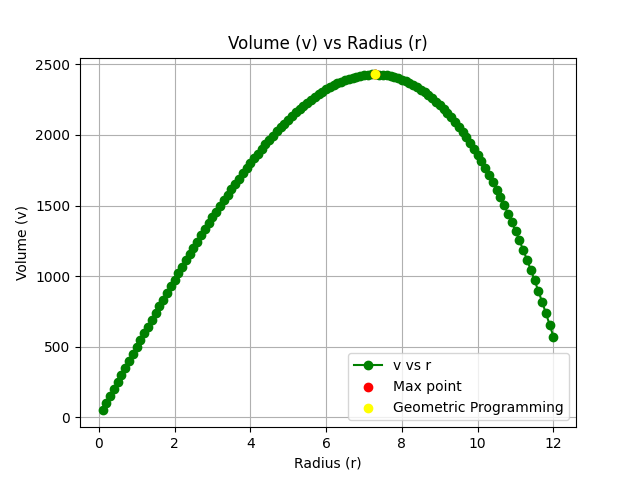
\includegraphics[width=0.8\textwidth]{figs/fig.png}
    \end{figure}
\end{frame}

\end{document}

